\section{Data Distribution Service for Data Exchange}
Data Distribution Service (DDS) is a messaging middleware standard \cite{dds-1.4-standard} for distributed applications governed by the Object Management Group (OMG).\footnote{\url{www.omg.org}} DDS is designed for mission- and business critical systems with real-time requirements. As such, it aims to function in a resource efficient, predictable and reliable manner, and is subject to minimal computational and transport overhead.
Thus, DDS is a great fit for the automotive use case. 

\subsection{Data-Centric Publish-Subscribe}
DDS is fundamentally based on the data-centric publish-subscribe (DCPS) communication paradigm. In the publish-subscribe-style communication, data flows between two kinds of entities: publishers and subscribers. Publishers provide data, while subscribers consume that data. A crucial characteristic of publish-subscribe is that data exchange between the peers is anonymous, \ie , publishers have no way of sending data to individual subscribers. Instead, both communicate by means of a shared, logical medium that takes data samples and forwards them to the appropriate receivers. In the context of DDS, this medium is called \emph{topic}. When subscribers receive a data sample they do not know where that sample originated. Similarly, publishers have no knowledge about where the sent data will end up at---or even if there are any receivers at all. Entities in this system find each other not by way of addressing, but rather on the basis of a shared understanding of what \emph{kind of data} they want to exchange. This approach is called \emph{data centricity}. Data centricity is in contrast to \emph{message centricity}, in which data exchange is driven by \emph{messages}, or \emph{instructions}, which are directed at individual receivers. A prominent example of a message-centric technology is Remote Procedure Call (RPC). To illustrate the difference between the two paradigms consider the example of a temperature sensor (henceforth also ``provider'') which propagates temperature data to multiple receivers (henceforth ``consumers'').

\paragraph{Message-Centric Approach.} In the message-centric paradigm, the temperature sensor transmits data samples encapsulated in \emph{messages} to the consumers. Messages are directed at each consumer individually, similar to a letter that is addressed to a certain postal address. This requires each participant to maintain their peers' location information (\ie\ their addresses) in local memory.
Two patterns are common in message-centric communication: ``push-based'', and ``pull-based'' (often ``request-reply''-style) communication~\cite{tanenbaum2017distributed}.

If message-centric communication is push-based, the sensor needs to know the addresses of all interested consumers a-priori. The provider thus has to maintain a list of consumers that it needs to update continuously. When a previously uninvolved consumer decides that it wants to receive temperature data, it first needs to register to the sensor in order to make its address known. The sensor then has to add the consumer's address to its list of consumers. Similarly, when a consumer is shut down, the sensor needs to remove the respective address, and has to deal with unexpected errors in case a consumer is suddenly unreachable. This (un)registration procedure is the cause of overhead and additional management effort, and makes the system inflexible and hard to scale. In contrast, pull-based communication don't rely on lists of consumers, but consumers request information from the provider. In this regard, pull-based communication is more scalable, however, additional overhead is incurred since two messages (instead of one) need to be transmitted for each data sample: a request and a response. Furthermore, consumers can not predict when a new data sample is available. The situation is made worse when there is not one producer, but many. Thus, both approaches are highly inefficient in the use case at hand.

\paragraph{Data-Centric Approach.} The DCPS approach, on the other hand, is exclusively push-based.\footnote{Although request-reply-style communication is not explicitly supported it can be mimicked (\cf \Cref{sec:ddslatency}).} The temperature sensor is a publisher in the publish-subscribe relationship, and the consumers are subscribers. A subscriber that is interested in the sensor's data only knows that it wants to receive \emph{temperature data}, \ie\ data samples of type ``temperature'', and thus, subscribes to the ``temperature'' topic. 
The temperature topic is defined by a unique identifier and a data type. Only data of that specific type may be published on the topic. To ease the use of the middleware, DDS provides typed interfaces to the exchanged data. Through the optional \emph{Data Local Reconstruction Layer} (DLRL) \cite{dlrl-1.4-standard}, data types can be defined via the DDS IDL,\footnote{``Interface Description Language''} and according language-specific stubs can be generated. The use of type safe interfaces not only improves usability, but also increases safety and error-proneness, as verifications can be performed at compile time.

In the temperature sensor example, the subscriber is entirely oblivious to the concept of \emph{temperature sensors}, or even if there are any sensors---it just listens in on the ``temperature'' topic. Similarly, the temperature sensor is only concerned with the provisioning of temperature data, and doesn't know which subscribers to send the data to. Thus, the temperature sensor publishes all samples it gathers on the ``temperature'' topic. If more temperature sensors were to be introduced to the system, they could simply be added by registering new publishers which would post data on the same topic. Since all publishers of a topic identify themselves purely on the basis of their topic, and not by their address or location, a great deal of redundancy can be achieved---all publishers of a given topic are entirely interchangeable.
Due to the agnostic relationship between publishers and subscribers, a high level of loose coupling is achieved. This allows for a simple extension of the system, making it extraordinarily scalable.

It is often helpful to think of publish-subscribe communication not in terms of messages that are sent from one entity to another, but rather as a \emph{shared global data space} in which data is universally accessible to all entities involved in the system. In this data space, each entity views data as if it were available in a local storage, when in reality, it is distributed among many other entities.

\subsection{Under the Hood}
Naturally, in order to realize a publish-subscribe system, addresses and locations of nodes are still crucial, as publish-subscribe, like other communication paradigms, rely on IP-based computer networks. This fact, however, is hidden behind the curtains of the middleware (DDS in this case). The middleware is responsible for the registration of publishers/subscribers, the dissemination of data to the appropriate receivers, and the enforcement of network reliability policies. In order to do this efficiently, the middleware maintains lists of subscribers, publishers and topics. Many middlewares employ central components called ``brokers'' for this. Depending on the view point and use case, the centralized nature of brokers may be considered advantageous, or disadvantageous. On the one hand, centralization is associated with simplicity since everything is managed in one spot, and only one single source of truth exists. On the other hand, this approach brings the danger of a single point of failure that causes the whole system to fail if the broker fails. Additionally, centralized brokers may introduce bottlenecks, inhibiting the scalability of the system. 
As DDS is strongly focused on scalability, DDS employs a \emph{brokerless} architecture in which the functionality of the communication system is distributed among all participating entities. Consequently, message delivery as well as service discovery is performed in a decentralized manner.
For this, DDS may optionally employ IP multicast, by which all communication is directed at dedicated multicast group addresses, instead of each node's individual address. The delivery of data is then the responsibility of the underlying infrastructure.

\subsection{Wire Protocol}
DDS, in itself, is only a standard. As such, DDS does not dictate, in detail, how to implement the concepts presented in the earlier sections. A number of DDS implementations from different vendors exist, all varying in terms of standard compliance, features beyond the standard, licensing, and other distinguishing factors. Compatibility between the respective implementations can be achieved by the use of the DDSI-RTPS\footnote{The ``DDSI'' in DDSI-RTPS is often omitted. The shortened form will henceforth be used.} (DDS Interoperability--Real-Time Publish-Subscribe) wire protocol, which all major implementations support. Although the RTPS protocol is directly related to DDS, its specifics are outsourced in a separate standard \cite{rtps-2.2-standard}.
As a wire protocol, RTPS is deliberately tailored to DCPS-style communication. As such, it supports reliable multicast-enabled data exchange and service discovery over unreliable and connectionless best-effort transports such as UDP/IP. Special emphasis is put on robustness, fault tolerance, scalability and performance. Thus, RTPS was conceptualized with safety-critical real-time applications in mind. Although RTPS is the preferred transport method for DDS applications, it is not the only option. Many DDS vendors support TCP, UDP, and shared memory for cases in which performance is critical.

%
%
%
%
%
%
%
%
%
%
%
%
%
%
\pagebreak
\subsection{DDS Components}
\begin{figure}[htpb]
  \centering
  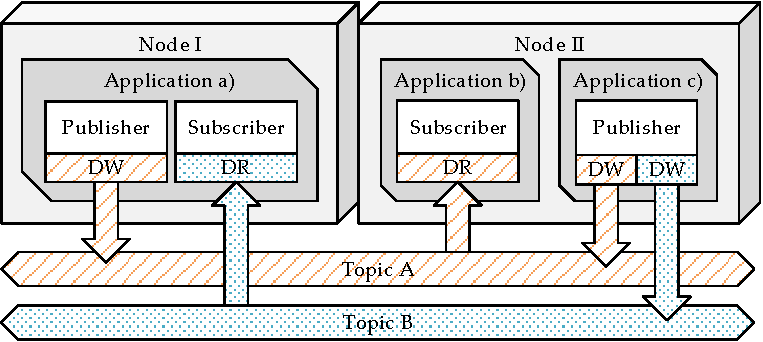
\includegraphics[width=0.8\textwidth]{figures/dds.pdf}
  \caption[An example of a distributed application connected via DDS]{An example of a distributed application connected via DDS}\label{fig:dds}
\end{figure}
The DDS specification defines a number of components which are introduced in the following. \Cref{fig:dds} depicts an example highlighting how the components are related. In the example, there are two hardware nodes connected by an unspecified computer network. Each node can execute multiple applications simultaneously. The applications communicate with each other by means of DDS.

\paragraph{Topics.}
\emph{Topics} form the basis on which peers communicate in the publish-subscribe paradigm. When a Publisher offers a certain kind of data, it does so by means of a Topic. When a data sample should be written, the Publisher pushes that data sample to a Topic appropriate for that sort of data. Conversely, when a Subscriber is interested in receiving data of a certain kind, then it subscribes to a Topic associated with that data. A Topic is uniquely defined by an identifier (name), a data type, and a set of QoS policies (see below). The data type represents the message format for data samples published on that Topic. For example, a suitable data type for a Topic concerned with temperature data would be a \texttt{struct} containing a single \texttt{float} value representing a temperature reading.
In \Cref{fig:dds} two Topics are depicted (Topic A and Topic B), each with a number of associated Data Writers and Data Readers (see below).

\paragraph{Publishers and Data Writers.}
\emph{Publishers} are entities that provide information in the publish-subscribe communication paradigm. Publishers are not bound to a single Topic. Instead, they contain one or more \emph{Data Writers}, each dedicated to a single Topic, who perform the actual data submission. Thus, Publishers may be seen as containers for a number of (unrelated) Data Writers. This concept is emphasized in \Cref{fig:dds} where a Publisher in Application c) controls two independent Data Writers that both write to different Topics.

\paragraph{Subscribers and Data Readers.}
\emph{Subscribers} are the exact compliment to Publishers in that they seek to receive data from Publishers. Analogous to Publishers, Subscribers are a way to group together sets of \emph{Data Readers}. Data Readers are entities whose purpose it is to receive data samples from their respective Topic. Through its API, DDS allows Data Writers to receive data in three ways: either by waiting for data samples (blocking the main thread), by pro-actively polling for new data samples, or by specifying asynchronous callbacks which are invoked whenever a data sample arrives.

\paragraph{Domains and Domain Participants.}
\emph{Domains} are the DDS way of grouping together sets of coherent \emph{Domain Participants} and to separate those sets from each other. Speaking in terms of distributed systems, Domains are a mechanism to manage group memberships of nodes \cite{tanenbaum2017distributed}. Domain Participants are entities that belong to a particular Domain. Each Publisher, Subscriber and Topic is derived from one Domain Participant and is therefore dedicated to exactly that Domain. As a consequence, participants of different Domains are entirely separated from each other and there is no way for them to interface with each other. Depicted in \Cref{fig:dds} is only one Domain. However, there could just as well be other Domains.


\subsection{Quality of Service}
One of DDS's salient features is its intrinsic support for Quality of Service (QoS), which is realized by so-called ``QoS policies''. QoS policies specify attributes that can be used to control each component's behavior and quality properties. They make specifying a component's behavior a matter of \emph{configuration}, rather than \emph{implementation}. For example, consider a Data Writer which writes data to a Topic at a high rate. A Data Reader may be interested in that data but not at such a high rate, \eg\ because it runs on an embedded device powered by a battery and therefore needs to manage power consumption carefully. The Data Reader may now apply a \tbf , which instructs DDS to block all samples that exceed a specified frequency threshold. This way, the rate of incoming messages can be controlled via configuration. This is beneficial for the programmer as they do not need to accommodate for this at code level, but let the middleware take care of it.

QoS policies can be set for each Topic, Publisher, Subscriber, Data Writer and Data Reader individually.
In \Cref{tab:qos}, an excerpt of the available QoS policies is given. For the exhaustive list of all available QoS policies refer to the official standard \cite{dds-1.4-standard}.

Another example of a QoS policy is the \deadline\ policy. It specifies the minimum sampling frequency of a Data Writer. If the deadline period of a hypothetical Data Writer is set to, e.g., 100 ms, then this Data Writer is obligated to send a data sample at least every 100 ms. If it fails to send samples at this rate, the Data Writer and all the respective Topic's readers will be notified about that circumstance and are free to act accordingly.

\begin{table}[H]
  \caption[An excerpt of DDS QoS policies]{An excerpt of QoS policies}\label{tab:qos}
  \centering
  \begin{tabular}{p{0.25\textwidth} p{0.2\textwidth}  p{0.45\textwidth}}
    \toprule
      \textbf{Name} & \textbf{Legal values} & \textbf{Description} \\
    \midrule
    	\reliability  & \texttt{RELIABLE}, \texttt{BEST\_EFFORT} & Indicates whether a Data Writer may drop samples or whether a Data Reader approves of Data Writers that drop samples.\\
    	\tbf  & An integer value denoting time & Specifies a Data Reader's desired data reception rate. Superfluous samples will be discarded.\\
    	\liveliness  & An integer value denoting time & Defines the rules to determine whether a particular entity is ``alive'', \eg\ by emitting heart beats. \\
    	\deadline  & An integer value denoting time & Establishes a contract between Data Writer and Data Reader to determine the acceptable data rate. \\
    	\ownership  & \texttt{SHARED}, \texttt{EXCLUSIVE} & Specifies whether multiple Data Writers may write to a given Topic simultaneously or just the one with the highest \ostrength\  value.\\
    	\ostrength  & An integer value denoting relative priority & Determines a Data Writer's priority in cases where its Topic's \ownership\ is set to \texttt{EXCLUSIVE}. \\
    \bottomrule
  \end{tabular}
\end{table}

In addition to specifying quality attributes, QoS policies may also serve as ``service contracts'' between interacting DDS components. These contracts specify non-functional requirements that the involved components must fulfill to be able to communicate with each other. For example, a Data Writer's \reliability\ policy may have been set to the \texttt{BEST\_EFFORT} level, thereby allowing the writer to drop samples. A Data Reader, on the other hand, may require the writer's policy to be set to \texttt{RELIABLE}, which prohibits the dropping of samples. Since the writer does not fulfill the reader's QoS requirements, the two components are considered incompatible, and thus, they cannot interact with each other.

Despite their name, QoS policies do not only concern \emph{quality} attributes per se. They can also be used to specify the priority of data samples, their lifespan, \ie , how long they are valid, or how many data samples of a certain type are kept in local memory.
%
%
%
%
%
%
%
%
%
%
%
%
\subsection{Redundancy and Automatic Failover} \label{sec:failover}
DDS has ways to ensure reliable communication---even over unreliable transmission channels. Part of reliability is failure transparency, \ie , the ability to quickly substitute failed components by backup components. The substitution process involves two steps: first, the failure needs to be detected. Second, a backup component needs to be instructed to take over. By means of the three QoS policies \ownership , \ostrength\ and \liveliness\ (\cf \Cref{tab:qos}), DDS may realize this process.

As the first step, a mechanism needs to determine whether a component has failed. In most cases, it is not possible for a failing component to properly shut down and ``sign off'', \ie , to notify the rest of the system that it will become unavailable. For this reason, the failure needs to be automatically registered. The \liveliness\ policy can be used to achieve this. \liveliness\ is the mechanism that determines whether a component is responsive (``alive''), or unresponsive (``dead''). The policy's value can be set to number indicating the maximum time interval between each liveliness signal. If a component fails to show a vital sign during that period, it is considered dead by the rest of the system. Passive components, \ie\ those which do not actively emit data, can be instructed to automatically send liveliness signals, or heartbeats, in certain intervals.

After a component has been declared dead it is up to the middleware to elect a substitute component. This is done through the \ownership\ and \ostrength\ QoS policies. By assigning a topic the \ownership\ value ``\qos{exclusive}'' one can specify that only a single data writer may write to that topic at any given time. Which data writer is given that prerogative is determined by the data writer's \ostrength\ value. The data writer that possesses the higher value is eligible to write to the topic. In the failover scenario, both, the primary data writer and the backup writer are assigned to the same topic, and both are configured to have exclusive \ownership\ rights. The former one has a higher \ostrength\ than the latter one. Based on both writer's \ostrength\ values, it is decided which one has precedence over the other.
%
%
%
%
%
%
%
%
%
%
%
%
%\subsection{Separation of User Data}
%The presented approach relies on a single cloud infrastructure, while at the same time, a vast number of customers need to be served. This poses a challenge concerning the separation of data. Confidentiality and privacy of user-specific application data must be preserved. Similarly, the result of a computation commissioned by a specific vehicle must be returned to exactly that vehicle, and no one else.

%Gladly, DDS offers a solution to this. In DDS, topics are not restricted to a single domain, \ie , they may be reused in multiple domains. If, \eg , a publisher belongs to \texttt{Domain $\alpha$} and publishes data on \texttt{Topic A}. Then, a data reader that reads from \texttt{Topic A} but belongs to \texttt{Domain $\beta$} may not read the data. Therefore, through domains, the same application may be reused several times on the same network, while keeping topic data separate. This principle is taken advantage of in the presented approach: domains are used to separate user data, such that for each user there is one user-specific domain. Thus, there is no way that data from one vehicle may interfere with data from another vehicle.

%\subsection{DDS for Automotive Systems}
%Automotive software systems have previously relied---and, to some degree, will continue to do so---on low-level, low-bandwidth transport protocols such as CAN, LIN, etc. For the longest time, networks stacks based on those protocols were sufficient to meet the basic requirements of delivering vehicular sensor data. However, driven by the emergence of innovative functions, the demands for vehicle intrinsic networks are skyrocketing. In particular, more and more sensor data from increasingly bandwidth-hungry sensors, such as cameras and lidars is feeding into advanced systems such as ADAS.
%At the same time, these functions require computational capabilities that go way beyond of what is possible with the microcontrollers typically used in traditional ECUs. High-performance computer systems based on high-level operating systems, supported by bandwidth-friendly networking protocols are needed to meet the new requirements.
%A new generation of low-level network protocols found their way into the vehicle. Notable mentions are FlexRay, and TSN. A question that remains is whether DDS is a suitable choice for the use within vehicles, and whether DDS may be used efficiently on top of these lower level protocols. \citeauthor*{bouhouch2013dds} have shown \cite{bouhouch2013dds} that DDS is indeed a suitable middleware to be used in vehicular networks.

%DDS allows to configure how much of a system's resources an DDS-enabled application may use. Consequently, it is the middleware's responsibility to allocate resources as needed while still staying within the specified boundaries. At the same time, priorities aligning with the application's QoS settings need to be considered. DDS takes this burden off the programmer's shoulders.
%\todo[inline]{TODO}


%
%
%
%
%
%
%
%
%
%
%
%
%
%
%
%
%
%
%
%
